
\chapter{Modelagem FrameWeb}
\label{sec-frameweb}
\vspace{-1cm}

\emph{\imprimirtitulo} é um sistema Web cuja arquitetura utiliza \textit{frameworks} comuns no desenvolvimento para esta plataforma. Desta forma, o sistema pode ser modelado utilizando a abordagem FrameWeb~\cite{souza-celebratingfalbo20}.

A Tabela~\ref{tabela-frameworks} indica os \textit{frameworks} presentes na arquitetura do sistema que se encaixam em cada uma das categorias de \textit{frameworks} que FrameWeb dá suporte. Em seguida, os modelos FrameWeb são apresentados para cada camada da arquitetura.

\begin{footnotesize}
	\begin{longtable}{|c|c|}
		\caption{\textit{Frameworks} da arquitetura do sistema separados por categoria.}
		\label{tabela-frameworks}\\\hline
		
		\rowcolor{lightgray}
		\textbf{Categoria de \textit{Framework}} & \textbf{\textit{Framework} Utilizado} \\\hline 
		\endfirsthead
		\hline
		\rowcolor{lightgray}
		\textbf{Categoria de \textit{Framework}} & \textbf{\textit{Framework} Utilizado} \\\hline 
		\endhead

		Controlador Frontal & {JSF} \\\hline

		Injeção de Dependências & {CDI} \\\hline

		Mapeamento Objeto/Relacional & {JPA} \\\hline

		Segurança & {JAAS} \\\hline
	\end{longtable}
\end{footnotesize}




\section{Camada de Negócio}
\label{sec-frameweb-negocio}

\begin{figure}[h]
    \centering
    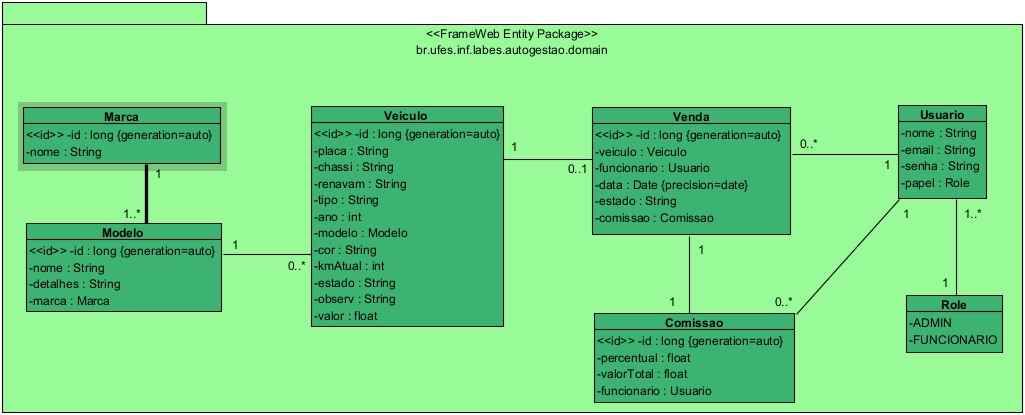
\includegraphics[width=0.8\textwidth]{figuras/Modelo de Entidades.jpg}
    \caption{Modelo de Entidades}
    \label{Modelo de Entidades.jpg}
\end{figure}


\section{Camada de Acesso a Dados}
\label{sec-frameweb-dados}

\section{Camada de Apresentação}
\begin{figure}
    \centering
    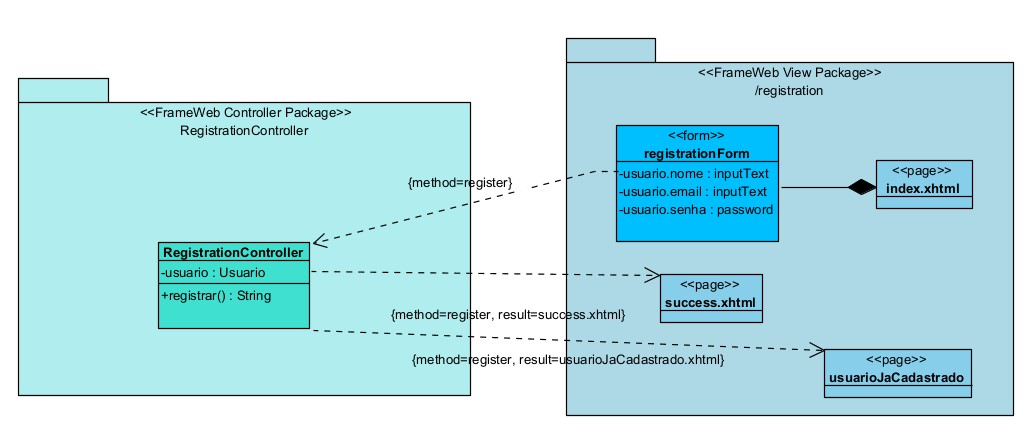
\includegraphics[width=0.9\textwidth]{figuras/Modelo de Navegacao 1.jpg}
    \caption{Modelo de Navegação 1 - Registro de usuário}
    \label{Modelo de Navegacao 1.jpg}
\end{figure}
\begin{figure}
    \centering
    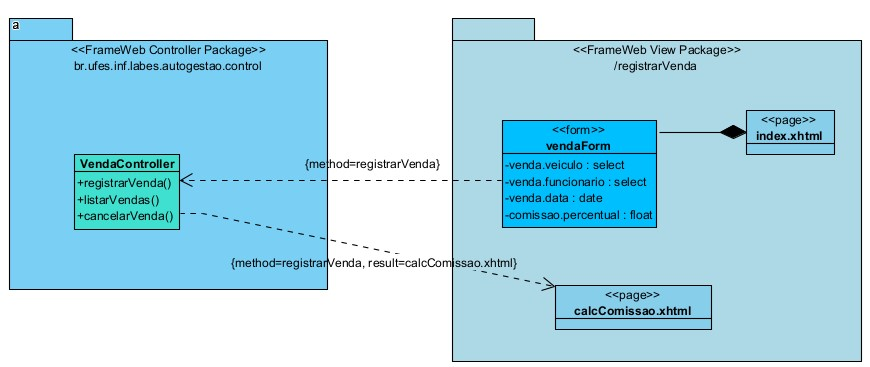
\includegraphics[width=0.9\textwidth]{figuras/Modelo de Navegacao 2.jpg}
    \caption{Modelo de Navegação 2 - Adicionar Venda}
    \label{Modelo de Navegacao 2.jpg}
\end{figure}